
\begin{figure}[H]
	\centering
	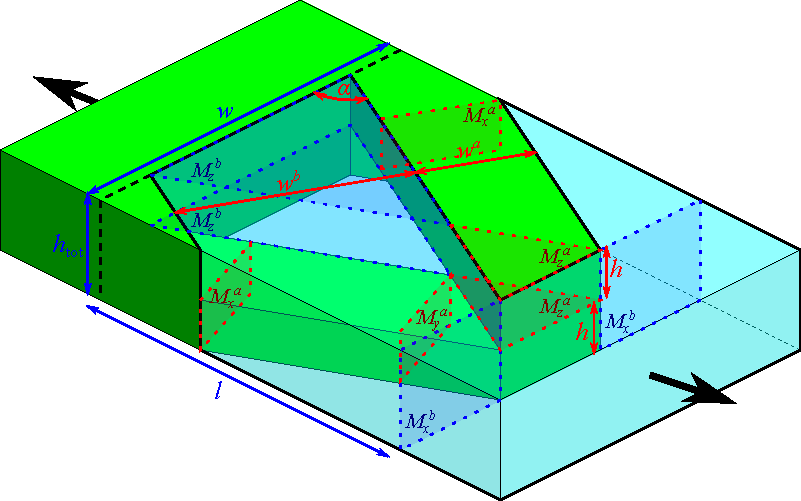
\includegraphics[width=\columnwidth]{sources/method/diagonal_model_v3.pdf}
	\caption{
		One diagonal unit cell connecting material $a$ (left) to material $b$ (right).
		Failure can happen along both the fingers ($M_x$), twice along one finger ($M_y$) or at the interface between the two fingers ($M_z$) for either material.}
	\label{fig:diagonal_model}
\end{figure}



\section{Diagonal Design}

Another option is to place the fingers under an angle as shown in \autoref{fig:diagonal_model}.
There are four design variables: the finger width of both materials: $w^a$ and $w^b$, the length $L$ and the layer thickness $h$.

\section{Problem Formulation}
\subsection{Geometry Relations}
From \autoref{fig:diagonal_model}, the geometry relations \ref{eq:tan}, \ref{eq:cos} and \ref{eq:sin} can be derived, which are used for further analysis of the stresses.

\begin{equation}
	\label{eq:tan}
	\tan \alpha = \frac{2L}{w_a + w_b}
\end{equation}

\begin{equation}
	\label{eq:cos}
	\cos \alpha = \frac{w_a + w_b}{\sqrt{ \left( w_a + w_b \right) ^2 + 4L ^2 }}
\end{equation}

\begin{equation}
	\label{eq:sin}
	\sin \alpha = \frac{2L}{\sqrt{ \left( w_a + w_b \right) ^2 + 4L ^2 }}
\end{equation}


\subsection{Tension Failure M$_x$}\label{ssec:tensfail}
For the tension failure, we consider the smallest cross sectional area of one finger, which is equal to $w_m h \sin \alpha$ . The tensile force perpendicular to this area is equal to $\frac{F}{\sin \alpha}$, where $F$ is the force per finger. %which was divided by 2 because every finger takes up half of the load. ? - adjust later maybe
Working out $\frac{F}{A} \le \sigma$ resulted in \autoref{eq:tensfail}


\begin{equation}
		\label{eq:tensfail}
	\frac{F}{w_m  h} \le \sigma_{max}
\end{equation}


\subsection{Shear Failure M\textsubscript{x}}
The same cross sectional area was taken as in \autoref{ssec:tensfail}, but now the force that is aligned with this cross section $F \cos \alpha$ is used to evaluate the shear forces. The maximum shear stress for a rectangular cross sectional area is equal to $\frac{3V}{2A}$. In this way, we derived \autoref{eq:shearfailtemp}

\begin{equation}
	\label{eq:shearfailtemp}
	\frac{3F \cos \alpha}{w_m h \sin \alpha} = \frac{3F }{w_m h \tan \alpha} \le \tau_m
\end{equation}

We plugged in \autoref{eq:tan} what resulted in \autoref{eq:shearmx}.
\begin{equation}
	\label{eq:shearmx}
	\frac{ 3 F \left(w_a + w_b \right) }{ 4  w_m h L} \le \tau_m	
\end{equation}

\subsection{Shear Failure M\textsubscript{z}}
For a triangular cross section, the maximum shear stress is equal to $\frac{3F}{bh}$, where $b$ and $h$ are the base and the height of the triangle. The width and height of the rectangular area that is loaded in shear are equal to $w_m$ and $\frac{w_m \tan \alpha}{2} $ respectively. Combining with \ref{eq:tan} gave \autoref{eq:shearMz}.

\begin{equation}
	\label{eq:shearMz}
	\frac{ 3 F \left(w_a + w_b \right) }{ w_m ^2 L} \le \tau_m	
\end{equation}


\subsection{Bending Failure M\textsubscript{x}}
The length of each finger, which we call $l$, is defined in \autoref{eq:l}

\begin{equation}
	\label{eq:l}
	l = \sqrt{ \frac{\left( w_a + w_b \right)}{2} ^2 + L^2 }
\end{equation}
Then we can derive the moment in \autoref{eq:momentder}.

\begin{equation}
	\label{eq:momentder}
	\frac{F \cos \alpha l}{2} =  \frac{F \frac{\left(w_a + w_b \right)}{2l} l}{2} = \frac{F \left(w_a + w_b\right)}{4}ent...
\end{equation}
The moment of inertia $I$ for the rectangular cross section is $\frac{h \left(w_m \sin \alpha \right)^3}{12}$. With $y = \frac{w_m \sin \alpha }{2}$, this gives a bending stress $\frac{M y}{I}$ as shown in \autoref{eq:bendingtemp}

\begin{equation}
	\label{eq:bendingtemp}
	\frac{3 F\left(w_a + w_b \right)}{2 h \left( w_m \sin \alpha \right)^2 } \le \sigma_m
\end{equation}

Then we replaced $\sin \alpha$ with \ref{eq:sin}, where \autoref{eq:bending} was the final result.

\begin{equation}
	\label{eq:bending}
	\frac{ 3 F \left(w_a + w_b \right) \left(\left(w_a + w_b \right) ^2 + 4L^2 \right)  }{ 8h w_m^2 L^2 }  \le \sigma_m
\end{equation}

\subsection{Von Mises Stress Criterion}
The tensile $\sigma_t$, bending $\sigma_b$ and shear stresses $\tau_x$ acting at the section $M_x$ were combined into the Von Mises stress criterion. The Von Mises stress is defined in \autoref{eq:vm}.

\begin{equation}
	\label{eq:vm}
	\sqrt{\frac{\left( \sigma_t + \sigma_b \right)^2}{2} + 3\tau_x ^2}
\end{equation}

We plugged in \autoref{eq:tensfail}, \ref{eq:shearmx} and \ref{eq:bending}, what gave \ref{eq:vmcrit}.

\begin{equation}
	\label{eq:vmcrit}
	\sqrt{\frac{1}{2} \left( \frac{F}{w_m  h} + 	\frac{ 3 F \left(w_a + w_b \right) \left(\left(w_a + w_b \right) ^2 + 4L^2 \right)  }{ 8h w_m^2 L^2 }   \right)^2+ 3\left(	\frac{ 3 F \left(w_a + w_b \right) }{ 4  w_m h L }  \right) ^2}
\end{equation}
\todo{How to put it on the page??} 


\subsection{Optimization Problem}
The goal is to maximize the strength while accounting for the failure modes in the constraints.
With that, the optimization problem can be formulated as follows:

\begin{align}
	f: & \max \frac{F}{2h \left(w_a + w_b\right)} \nonumber \\
	\text{subject to:} & \nonumber \\
	g_1: & w_m \ge w_\text{m,min} \\
	g_2: & w_a + w_b \le w_\text{max} \\
	g_3: & L_{min} \le L \le L_{max} \\
	g_4: & h \ge h_{min} \\
	g_5: & \frac{ 3 F \left(w_a + w_b \right) }{ w_m ^2 L} \le \tau_m						\text{ Shear failure } M_z^m \\
	g_6:& \sqrt{\frac{1}{2} \left( \frac{F}{w_m  h} + 	\frac{ 3 F \left(w_a + w_b \right) \left(\left(w_a + w_b \right) ^2 + 4L^2 \right)  }{ 8h w_m^2 L^2 }   \right)^2+ 3\left(	\frac{ 3 F \left(w_a + w_b \right) }{ 4  w_m h L}  \right) ^2}		\le 	\sigma_m	\text{ Von Mises criterion } M_x \\
	& \text{for both materials } && m \in \{a, b\} \nonumber 
\end{align}


Normalizing and rewriting to the negative null-form gives the following optimization problem:

\begin{align}
	f: & \min \frac{2h \left(w_a + w_b\right)}{F} \nonumber \\
	\text{subject to:} & \nonumber \\
	g_{1a}:& 1 - \frac{w_a}{w_{a,min}}  \le 0 \\
	g_{1b}:& 1 - \frac{w_b}{w_{b,min}}  \le 0 \\
	g_2:& \frac{w_a + w_b}{w_{max}}  - 1 \le 0 \\
	g_{3.1}:& 1 - \frac{L}{L_{min}} \le 0 \\
	g_{3.2}:&\frac{L}{L_{max}} - 1  \le 0 \\
	g_4:& 1 - \frac{h}{h_{min}} \le 0 \\
	g_{5a}: & \frac{ 3 F \left(w_a + w_b \right) }{ \tau_a w_a ^2 L} - 1 \le 0					\text{ Shear failure } M_z^a \\
	g_{5b}: & \frac{ 3 F \left(w_a + w_b \right) }{ \tau_b w_b ^2 L} - 1 \le 0					\text{ Shear failure } M_z^b \\
	g_{6a}:& \frac{\sqrt{\frac{1}{2} \left( \frac{F}{w_a  h} + 	\frac{ 3 F \left(w_a + w_b \right) \left(\left(w_a + w_b \right) ^2 + 4L^2 \right)  }{ 8h w_a^2 L^2 }   \right)^2+ 3\left(	\frac{ 3 F \left(w_a + w_b \right) }{ 4  w^a h L}  \right) ^2}	} { \sigma_a} - 1	\le 0	\text{ Von Mises criterion } M_x^a \\
	g_{6b}:& \frac{\sqrt{\frac{1}{2} \left( \frac{F}{w_b  h} + 	\frac{ 3 F \left(w_a + w_b \right) \left(\left(w_a + w_b \right) ^2 + 4L^2 \right)  }{ 8h w_b^2 L^2 }   \right)^2+ 3\left(	\frac{ 3 F \left(w_a + w_b \right) }{ 4  w^b h L}  \right) ^2}	} { \sigma_b} - 1	\le 0	\text{ Von Mises criterion } M_x^a 
\end{align}
\todo{How to put it neatly on one line?}


\section{Initial Problem Investigation}

\subsection{Boundedness}

\subsection{Convexity}

\subsection{Monotonicity}
\begin{align}
	f: & F^-, h^+, w_a^+, w_b^+ \\
	g_{1a}:& w_a^- \\
	g_{1b}:& w_b^- \\
	g_{2}:& w_a^+, w_b^+\\
	g_{3.1}:& L^- \\
	g_{3.2}:& L^+ \\
	g_{4}:& h^-\\
	g_{5a}:& F^+, w_a^-, w_b^+, L^- \\
	g_{5b}:& F^+, w_a^+, w_b^-, L^-\\
	g_{6a}:& F^+, h^-, w_b^+, L^-\\
	g_{6b}:& F^+, h^-, w_a^+, L^-
\end{align}

\subsection{Numerical Noise}

\subsection{Sensitivity Analysis}



\section{Initial Optimization}

\section{Optimization of the Actual Problem}

